\documentclass[a4paper, 11pt]{article}
\usepackage[left=2.5cm,right=2.5cm,top=3cm,bottom=3cm,a4paper]{geometry}
\usepackage{kotex}
\usepackage{color}
\usepackage{enumitem}
\usepackage[cmyk, dvipsnames, svgnames]{xcolor}
\usepackage{graphicx}
\DeclareGraphicsExtensions{.pdf,.png,.jpg}
\usepackage[onehalfspacing]{setspace}
\setstretch{2.0}
\usepackage[colorlinks,urlcolor=blue,filecolor=magenta]{hyperref}
\usepackage{url}
\usepackage{graphicx,subfigure}






\title{\textbf{\Huge오목 한글 설명서}}
\author{\textbf{\LARGE5조}}
\begin{document}
	
	\maketitle
	
	\vspace{6cm}
	\begin{center}
		\textbf{\large20134824김민석}\\
		\textbf{\large20134852허정건}\\
		\textbf{\large20134867이현문}\\
	\end{center}
	
	
	
	
	\maketitle
	\newpage
	\thispagestyle{empty}        
	\mbox{}
		
	\begin{center} 
		\textbf{\Huge목차}\\
	\end{center}
	\vspace{0.5cm}
\section{프로그램 선택 이유}
	\vspace{0.5cm}
	\section{프로그램 설명}
	\begin{itemize}
		\item 소개 및 목표
	\end{itemize}
	
	\section{게임 소개}
		\begin{itemize}
		\item 각 실행 화면
	\end{itemize}

	
	\section{기능 설명}
	\begin{enumerate}
		\item a설명
		\item b설명
		\item c설명
	\end{enumerate}
	
	
	
	
	\section{버그}
	
	\vspace{0.5cm}
	\section{개선할 점}

	
	\vspace{0.5cm}
	\section{GitHub 협력자료}
	
   \newpage
	\title{\textbf{\Huge1. 프로그램 선택 이유}}\\
	
\textbf{	{\Large
		\begin{itemize}
			\item 현재 수 많은 오픈소스중에 설명서를 만듦에 있어 평소 우리가 자주 사용하지 않는 프로그램 보다 더 익숙하고 쉽게 접근할 수 있는 프로그램을 찾아 설명서를 만들어 보자는 생각에서 부터 오픈소스를 찾게되었다.
			\item 평소 게임을 좋아하는 우리 팀은 자연스럽게 게임에 대한 오픈소스를 찾게되었고 그로부터 우리나라의 전통놀이인 오목게임의 오픈소스를 찾게되었다. 누구나 쉽고 익숙하게 즐길 수 있는 전통놀이 오목의 설명서를 만들면서 오목게임도 할 수 있고,설명서를 만들어 다른 사람에게 도움도 줄 수 있어 일석이조라고 생각하여  이 프로그램을 선택하게 되었다.
		\end{itemize}
	}
	}


	\newpage
	\title{\textbf{\Huge2. 프로그램 설명}}\\
	\textbf{
	\begin{itemize}
		\item \LARGE소개 
	\end{itemize}
	{\Large
	본 프로그램은 네이버 블로거 dnpc7848 에 의해 개발 되었으며, 현재 모든 소스를 오픈하고 수정과 배포에 제한을 두지 않고 있다.\\
	현재 다음 링크에서 쉽게 다운로드 받아 사용, 수정이 가능하다\\
	\url{http://blog.naver.com/dnpc7848/220895826336}
	}
	\begin{itemize}
		\item \LARGE목표
	\end{itemize}
	{\Large
		본 프로그램에서 일반 룰, 고모쿠 룰, 렌주 룰  이 세 가지 룰에 대해 각 룰을 선택하여 실행하고, AI 모드를 통해 인공지능 상대와 게임을 즐기며 또한 남녀노소 가리지 않고 누구나 쉽게 오목을 접하여 배우기 위함에 목표를 둔다
	}}
	\newpage
	\title{\textbf{\Huge3. 게임 소개}}\\
\begin{figure}[h] %%% t: top, b: bottom, h: here
	\begin{center}
		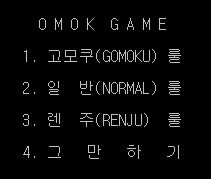
\includegraphics[width=0.5\linewidth]{first.png}
	\end{center}
	\label{fig:long}
	\label{fig:onecol}
\end{figure}
\begin{center}
	\textbf{{\Large 1. 룰 선택 화면\\}}
	\textbf{{\normalsize 원하는 룰 선택 \\}}
	\vspace{1.5cm}
\end{center}

\begin{figure}[h] %%% t: top, b: bottom, h: here
	\begin{center}
		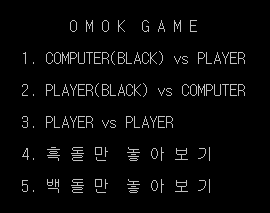
\includegraphics[width=0.5\linewidth]{second.png}
	\end{center}
	\label{fig:long}
	\label{fig:onecol}
\end{figure}
\begin{center}
	\textbf{{\Large 2. 플레이어 선택 화면\\}}
	\textbf{{\normalsize 원하는 상대 선택 \\}}
\end{center}

	\newpage
\begin{figure}[h] %%% t: top, b: bottom, h: here
	\begin{center}
		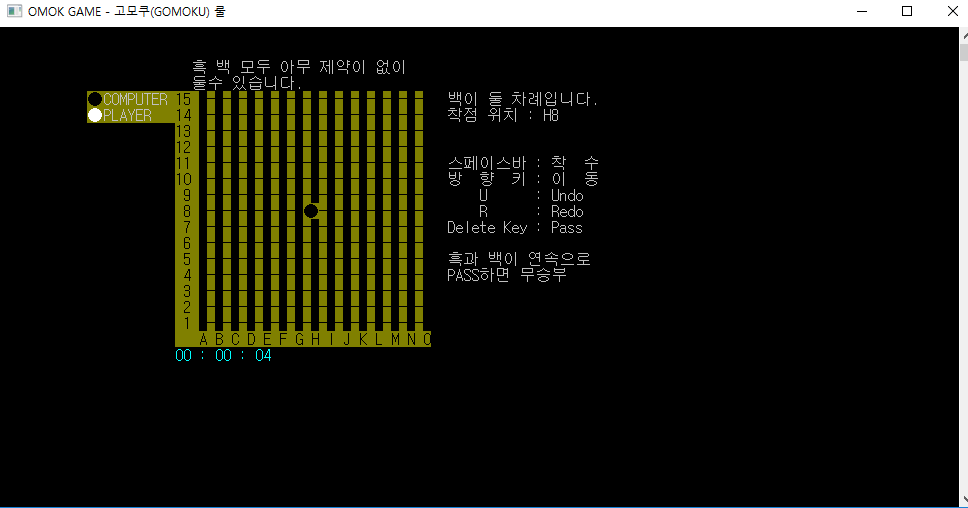
\includegraphics[width=0.8\linewidth]{third.png}
	\end{center}
	\label{fig:long}
	\label{fig:onecol}
\end{figure}
\begin{center}
	\textbf{{\Large 3. 게임 실행 화면\\}}
	\textbf{{\normalsize 게임 시작! \\}}
	\vspace{0.5cm}
\end{center}

\begin{figure}[h] %%% t: top, b: bottom, h: here
	\begin{center}
		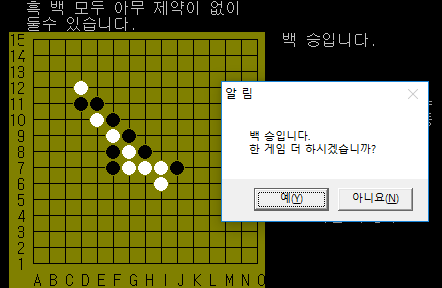
\includegraphics[width=0.8\linewidth]{4th.png}
	\end{center}
	\label{fig:long}
	\label{fig:onecol}
	
\end{figure}

\begin{center}
	\textbf{{\Large 4. 게임 결과\\}}
	\vspace{0.3cm}
	\textbf{{\normalsize 이겼닭! \tiny 오늘 저녁은 치킨이닭!  \\}}
\end{center}

 \newpage
\title{\textbf{\Huge4. 게임 룰 설명 및 조작법 }
	\vspace{0.5cm}
	\\ 1)게임룰
	
	\begin{figure}[h] %%% t: top, b: bottom, h: here
		\begin{center}
			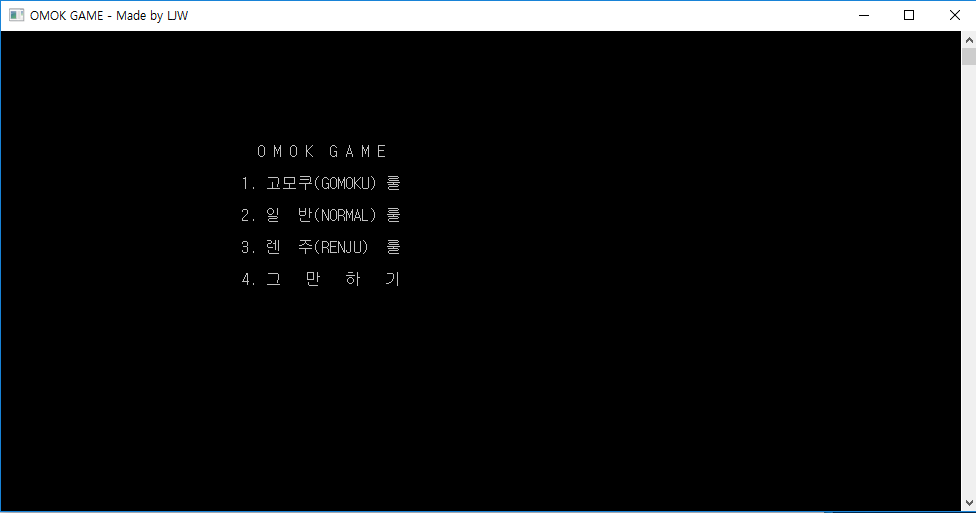
\includegraphics[width=1.0\linewidth]{OM1.png}
		\end{center}
		\caption{게임 실행시 룰 선택}
		\vspace{0.5cm}
		\ 오목게임실행시 첫 화면으로 고모쿠룰 일반룰 렌주룰 3가지중 하나의 룰을 선택합니다. (이걸 외부 기능으로 옮겨야 할듯)
	\end{figure}
	
	\newpage
	\begin{figure}[h]
		\begin{center}
			\subfigure{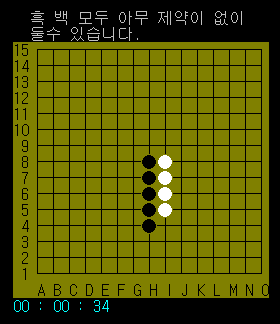
\includegraphics[width=0.35\linewidth]{komoku.png}}
			\\ 고모쿠룰 :  아무런 제약이 없는 오목으로, 먼저 두는 흑돌 에게 유리하다. 백돌 에게 불공평하기 때문에 공식에서 잘 쓰이지 않는다. 
			
			\vspace{1.5cm} 	
			
			
			\subfigure{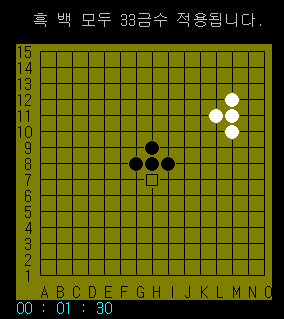
\includegraphics[width=0.35\linewidth]{normal.png}}
			\\ 일반룰 : 일상적으로 가볍게 대전할 때 가장 많이 사용되는 룰이다. 일단 3-3은 흑, 백 모두 금지되나 여기서 2개의 라인의 양 끝, 즉 4개의 끝 중 하나라도 막혀있으면 금지수가 아니다. 4-4에서 4가 하나 띄워져 있더라도 금지이다.
		\end{center}
	\end{figure}
	
	\newpage
	\begin{figure}[h] %%% t: top, b: bottom, h: here
		\begin{center}
			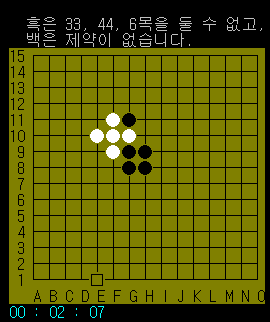
\includegraphics[width=0.35\linewidth]{renju.png}
			\\ 렌주룰 : 국제적인 룰로 흑만 3-3과 4-4, 장목이 금지하고, 백은 허용한다. 물론 금수와 함께 5도 만들어지는 경우에는 흑 승리로 한다.
		\end{center}
	\end{figure}
	
	
	\newpage
	\title{게임조작법}
	\begin{figure}[h] %%% t: top, b: bottom, h: here
		\begin{center}
			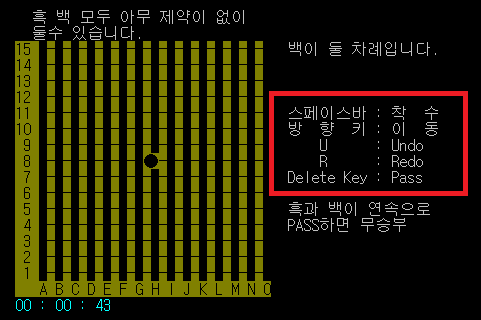
\includegraphics[width=0.5\linewidth]{OM_5.png}
		\end{center}
		\vspace{0.5cm}
		\ 스페이스바 : 놓기
		\\ 방향키 : 이동
		\\ 무르기 : U
		\\ 다시하기 : R
		\\ 턴넘기기 : Delete Key
	\end{figure}
 \newpage
\title{\textbf{\Huge5. 버그 }
	
		\vspace{1cm}
	{\large
\textbf{1. 구현된 3가지 룰을 선택해도 모두 '일반 룰'로 진행되는 버그}
	
\textbf{2. 게임 결과 창  표시 후 첫 화면으로 돌아가는 것이 아닌 프로그램 종료 현상.}
	
\textbf{3. 육(6)목 이상을 나열 한 경우, 룰을 무시하고 승리로 간주되는 현상 }
	
\textbf{4. 조작키 설명 중 U(Undo)와 R(Redo) 둘다 같은 '되돌리기' 기능을 수행하면서}
  \textbf{\quad 각각 다른 키로 구현}
 	
\textbf{5. 첫 화면으로 되돌아가는 'ESC' 기능이 룰 선택 화면에서는 적용이 되지않음}
}
	\vspace{3cm}

	\title{\textbf{\Huge6. 개선점 }
		
	\vspace{1cm}
		
	{\large		
\textbf{ 1. 게임 시작시 항상 시작 돌이 H8 위치가 아닌 랜덤위치에서 시작 될 수 있게 수정}
		
\textbf{2. 결과 화면 승리자  '흑돌 승' 대신, 사용자 승리 로 표시}
		
\textbf{3. 조작키 설명 중 Delete Key 기능인 PASS를 더 쉽게 이해하기 위해 DRAW로 수정 }
		
\textbf{4. 제한시간을 두어 게임에 긴장감 조성이 필요}
		
\textbf{5. 마지막으로 둔 돌 위치를 강조하여 헷갈리지 않게 할 필요}
}

\newpage

	\title{\textbf{\Huge7. GitHub 협력자료 }
\end{document} 